\documentclass{article}
\usepackage[margin=1in]{geometry}
\usepackage{tikz}
\usepackage{amsmath}
\usepackage{setspace}

\begin{document}
\title{Calculations for JMTSCADLIB}
\author{JimmyMadeThat}
\maketitle

\section{Functions}

\subsection{Height of Sloped Cylinder}

Given a bottom radius ($r_1$), top radius ($r_2$), and slope ($\theta$, where 90° is a vertical/unsloped and 0° is a completely flat circle), determine the height ($h$) of the cylinder.

\begin{figure}[h!]
\centering
\begin{tikzpicture}
    \draw (0,0) -- (1,6) -- (5,6) -- (6,0) -- cycle;
    \draw (3,0) -- (3,6);
    \draw (3,-0.5) -- (6,-0.5);
    \draw[dotted] (5,0) -- (5,6);
    \draw (5,0.2) -- (5.2,0.2) -- (5.2,0);

    \draw (4,6) node[above] {$r_2$};
    \draw (4.5,-0.5) node[below] {$r_1$};
    \draw (5.5,0) node[below] {$r_d$};
    \draw (5.8, 0.2) node {$\theta$};
    \draw (5, 3) node[left] {$h$};
\end{tikzpicture}
\caption{Side view of sloped cylinder}\label{fig:sloped_cylinder}
\end{figure}

Adding the value $r_d$, equaling $r_1 - r_2$, we solve for $h$:

\begin{align*}
    \tan(\theta) &= \frac{h}{r_d} && \text{SOHCAH\textbf{TOA}} \\
    h &= r_d \tan(\theta) && \text{Multiply by $r_d$, switch sides} \\
    h &= (r_1 - r_2) \tan(\theta) && \text{Substitute $r_d$}
\end{align*}

\subsection{Packed Field of Circles}

Given a radius ($r$), maximum width in x direction ($w_{max}$), maximum depth in y direction ($d_{max}$), pack circles to fill (but not overflow) the area. Then calculate the actual width ($w_{actual}$), actual depth ($d_{actual}$), number of columns ($c$), number of rows in odd-numbered columns ($n_{odd}$), and number of rows in even-numbered columns ($n_{even}$). This relationship is shown in Figure~\ref{fig:packed_circles_layout}.

\begin{figure}[h!]
\centering
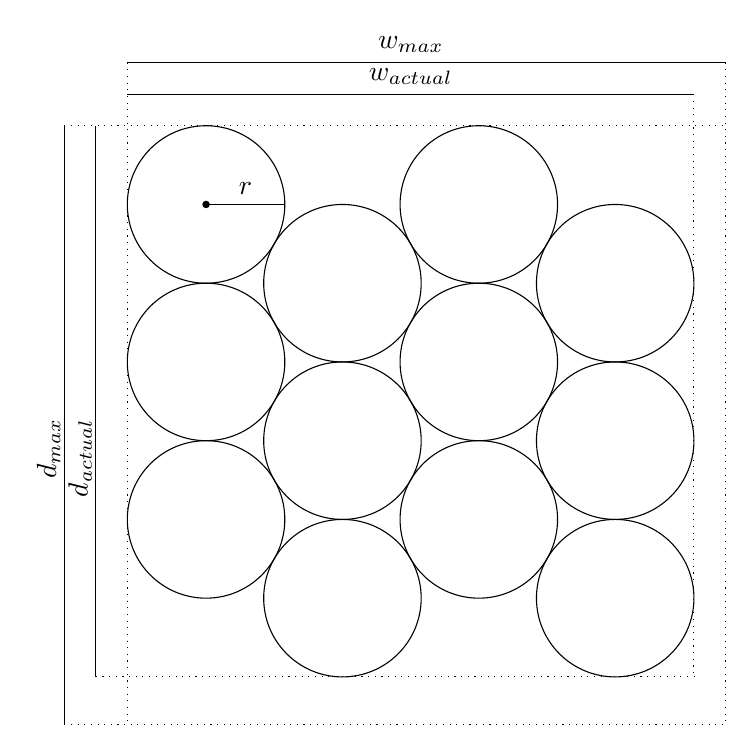
\begin{tikzpicture}[scale=0.4]

% Circles
\draw (2.5, 5.5) circle (2.5);
\draw (2.5, 10.5) circle (2.5);
\draw (2.5, 15.5) circle (2.5);
\draw (6.83, 3) circle (2.5);
\draw (6.83, 8) circle (2.5);
\draw (6.83, 13) circle (2.5);
\draw (11.16, 5.5) circle (2.5);
\draw (11.16, 10.5) circle (2.5);
\draw (11.16, 15.5) circle (2.5);
\draw (15.49, 3) circle (2.5);
\draw (15.49, 8) circle (2.5);
\draw (15.49, 13) circle (2.5);

% Top-left circle radius
\filldraw (2.5,15.5) circle (0.1);
\draw (2.5,15.5) -- (5,15.5);
\draw (3.75,15.5) node[above] {$r$};

% Width labels
\draw (0,19) -- (17.99,19);
\draw (0,20) -- (19,20);
\draw (9,19) node[above] {$w_{actual}$};
\draw (9,20) node[above] {$w_{max}$};
\draw[dotted] (0,20) -- (0,-1);
\draw[dotted] (19,20) -- (19,-1);
\draw[dotted] (17.99,19) -- (17.99,0.5);

% Depth labels
\draw (-1,18) -- (-1,0.5);
\draw (-2,18) -- (-2,-1);
\draw (-1.5,9) node[left, rotate=90] {$d_{actual}$};
\draw (-2.5,9) node[left, rotate=90] {$d_{max}$};
\draw[dotted] (-1,0.5) -- (17.99,0.5);
\draw[dotted] (-2,-1) -- (19,-1);
\draw[dotted] (-2,18) -- (19,18);

\end{tikzpicture}
\caption{Layout of packed circle field}\label{fig:packed_circles_layout}
\end{figure}

To determine $c$, $n_{even}$ and $n_{odd}$, we need to express $w_{actual}$ and $d_{actual}$ in terms of $r$ and these target variables. Figure~\ref{fig:packed_circles_rel_w} shows this relationship for width and TODO shows this relationship for depth.

\begin{figure}[h!]
\centering
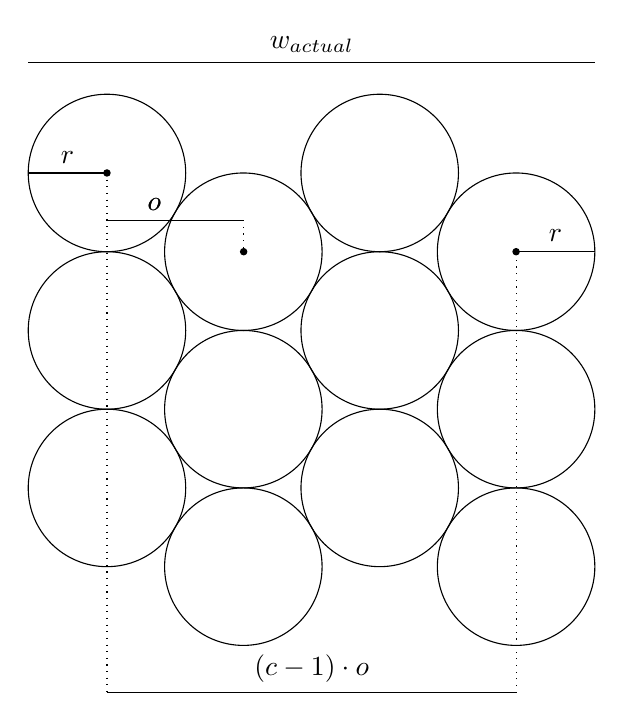
\begin{tikzpicture}[scale=0.4]

% Circles
\draw (2.5, 5.5) circle (2.5);
\draw (2.5, 10.5) circle (2.5);
\draw (2.5, 15.5) circle (2.5);
\draw (6.83, 3) circle (2.5);
\draw (6.83, 8) circle (2.5);
\draw (6.83, 13) circle (2.5);
\draw (11.16, 5.5) circle (2.5);
\draw (11.16, 10.5) circle (2.5);
\draw (11.16, 15.5) circle (2.5);
\draw (15.49, 3) circle (2.5);
\draw (15.49, 8) circle (2.5);
\draw (15.49, 13) circle (2.5);

% Top-left circle radius
\filldraw (2.5,15.5) circle (0.1);
\draw (0,15.5) -- (2.5,15.5);
\draw (1.25,15.5) node[above] {$r$};

% Top-right circle radius
\filldraw (15.49,13) circle (0.1);
\draw (15.49,13) -- (17.99,13);
\draw (16.74,13) node[above] {$r$};

% O markers
\draw[dotted] (2.5, 15.5) -- (2.5, -1);
\draw[dotted] (6.83, 14) -- (6.83, 13);
\draw[dotted] (15.49, -1) -- (15.49, 13);
\draw (4,14) node[above] {$o$};
\filldraw (6.84,13) circle (0.1);
\draw (2.5, 14) -- (6.83, 14);
\draw (4,14) node[above] {$o$};

% Width labels
\draw (0,19) -- (17.99,19);
\draw (9,19) node[above] {$w_{actual}$};
\draw (2.5,-1) -- (15.49,-1);
\draw (9,-1) node[above] {$(c-1) \cdot o$};

\end{tikzpicture}
\caption{Width relationship between $w_{actual}$, $r$, $c$, and an unknown overlap value $o$}\label{fig:packed_circles_rel_w}
\end{figure}

In the width relationship (Figure~\ref{fig:packed_circles_rel_w}), an unknown variable, $o$, represents the width of the overlap between the columns of circles.

\begin{figure}[h!]
\centering
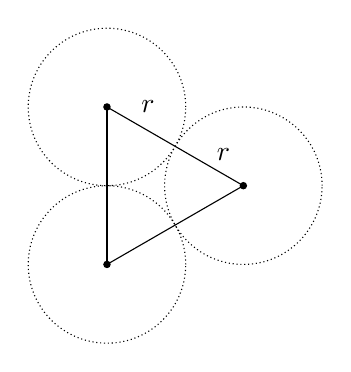
\begin{tikzpicture}[scale=0.4]

% Circles
\draw[densely dotted] (2.5, 10.5) circle (2.5);
\filldraw (2.5,10.5) circle (0.1);
\draw[densely dotted] (2.5, 15.5) circle (2.5);
\filldraw (2.5,15.5) circle (0.1);
\draw[densely dotted] (6.83, 13) circle (2.5);
\filldraw (6.83,13) circle (0.1);

% Top-left circle radius
\draw (2.5,15.5) -- (6.83,13);
\draw (2.5,10.5) -- (6.83,13);
\draw (2.5,10.5) -- (2.5,15.5);
\draw (3.8,15) node[above] {$r$};
\draw (6.2,13.5) node[above] {$r$};

\end{tikzpicture}
\caption{Relationship between $o$ and $r$}\label{fig:packed_circle_triangle}

\end{figure}
\end{document}
